% Comments:
% Why use session types? The advantages
% Maybe have an untyped commitment protocol
% Benefit of session types: extra type annotations, concise specification
% Does not provide a complete term, only a specification
% Might make sense to talk about extending session types with dependencies for commitment

%Just like distributed protocols, cryptographic protocols follow a predefined communication pattern.
Our central focus in this work is exploring the role of \emph{session} types in defining and analyzing ideal functionalities.
Expressing bi-directional communication in the type systems reveals more information to a programmer of what a protocol or ideal functionality does, and enforcing it statically eases the programming burden of writing ``correct'' code.\todo{correct here in terms of using the functionality or protocol correctly}
In this section, we illustrate how session types can be used to describe protocol interfaces, what information is leaked to the adversary, and, as we'll see in a later section, what its runtime requirements are.
%We do so and introduce our running example throughout the paper: a simple, linear database functionality, \Fdb
We do so through a running example we will use throughout this paper, the cryptographic commitment functionality \Fcom.

\paragraph{The Ideal Bit Commitment}
The ideal functionality \Fcom is a straightforward primitive that underlies many important and widely used protocols. 
The version presented in Figure~\ref{fig:fcom} allows a sender $S$ commit to a single bit $b$ and reveal it later to a receiver $R$.
It asserts two properties: \emph{binding} and \emph{hiding}.
Binding guarantees that $S$ can't flip the bit that was committed to, and hiding guarantees that $R$, or the adversary, learns nothing about the $b$ until it is revealed.
\Fcom also leaks to the adversary that the commitment has been made.
This leaks is absolutely necessary, because it quantifies what the adversary allowed to learn in a protocol that will realized \Fcom. 
If \Fcom leaks no information, then no simulator proof will be possible for any real-world protocol is the two parties are both honest.

\begin{figure}
\begin{minipage}{0.38\textwidth}
\begin{bbox}[title={Functionality $\F_{\m{com}}(S, R)$}]\\
\textbf{on input} \inmsg{\m{Commit}}{$b$} from $S$:\\
\hspace*{1em} store $b$;\\
\hspace*{1em} output (\m{Committed}) to $R$.\\ \\
Then, \textbf{on input} \inmsg{\m{Open}} from $S$:\\
\hspace*{1em} send $(\m{Open}, b)$ to $R$.
\end{bbox}
\end{minipage}
\hspace{3em}
\begin{minipage}{0.5\textwidth}
\begin{lstlisting}[basicstyle=\scriptsize\BeraMonottFamily, frame=single, mathescape, numbers=left]
$\nproc$ $\tm{Fcom}$: 
(k: $\tgr{int}$), (rng: [Bit]), (sid: SID),
(S: sender), (R: receiver)  |- (fc: 1) =
{
  $\ncase$ S (
    Commit => b = $\nrecv$ S ;
              R.Committed ;
              $\ncase$ S (
                Open => R.Open ;
                        $\nsend$ R b ;
              )
  )
}
\end{lstlisting}
\end{minipage}
\caption{(a) Pseudocode for a one-shot \Fcom parameterized by a sender $S$ and receiver $R$,
and (b) the corresponding code in NomosUC}
\label{fig:fcomideal}
\vspace{-4mm}
\Description{Ideal Fcom}
\end{figure}


Our description of the commitment is summarized by the following binary session types that outline the communication between \Fcom and each of $S$, $R$, and \A.
These same types will exist in the real world between \Z and each of $S$ and $R$.

\scalebox{0.9}{
\begin{mathpar}
  \mi{type} \; \m{sender} = \textcolor{red}{\getpot^2} \ichoice{\mb{commit} : \m{bit} \product \ichoice{\textcolor{red}{\getpot^0}\mb{Open} : \one}}
\end{mathpar}
}
\scalebox{0.9}{
\begin{mathpar}
  \mi{type} \; \m{receiver} = \textcolor{red}{\paypot^1} \echoice{\mb{rcommit} \arrow \echoice{\textcolor{red}{\paypot^0}\mb{ropen}: \m{bit} : \one}}
\end{mathpar}
}
\scalebox{0.9}{
\begin{mathpar}
  \mi{type} \; \m{adv} = \echoice{\mb{acommit}: \ichoice{\mb{ok}: \one}}
\end{mathpar}
}

Binary session types are defined via two type constructors, $\ichoice$ (internal choice) and $\echoice$ (external choice). 
They determine which of the two processes can send a message.
The sender's choice above only uses $\ichoice$ because \Fcom never gives it any output, and the receiver's type only uses $\echoice$.
At any given moment only one of $\ichoice$ or $\echoice$ can be valid, meaning only one of the two endpoints of the channel can send a message on it.
For cases where non-determinism is needed and either endpoint can send a message, communication can be split over multiple channels as necessary.
To begin a commitment $S$ sends the label \m{commit} over its the channel along with a \m{Bit} to commit to.
\Fcom alerts \A with the label \m{acommit} and waits for it to return with an \m{ok} before telling the receiver with \m{rcommit}.
Finallty, $S$ opens the commitment the label \m{open}, and \Fcom sends \m{ropen} a long with the originally committed bit $b$ to $R$.
A notable restriction here is that the session types above only define communication between pairs of parties and don't enforce that $S$ must commit before \Fcom can send \m{rcommit} to $R$.
\todo{revise the point about polymorphism here}

In the real-ideal paradigm, we compare two worlds each with its own protocol.
The ideal world consits of \Fcom along with a dummy protocol where parties forward all communication between \Z and the functionality.
The dummy protocol provide the same session types as used by \Fcom, and, therefore, the real world where parties locally run \protcom also exhibi the same type.

% \centering
\begin{bbox}[title={Functionality $\F_{\m{RO}}$}]
~
Initialize empty table $\ell \leftarrow \emptyset$\\
\qquad -- On input \inmsg{\m{query}}{$x$} from $P_i$: send $h'$ to $P_i$;\\
\qquad if $(x,h')$ exists in $\ell$, else add $(x, h \xleftarrow{\$}\{0,1\}^k)$ to $\ell$\\
\qquad and send it to $P_i$

\end{bbox}
\vspace{-0.5em}
\caption{Pseudocode for the random oracle.}
\label{fig:fro}


\paragraph{Random Oracle}
The commitment protocol \protcom that realize \Fcom operates in the random oracle model. 
The the random oracle model assumess protocol parties have access to an idealized hash function \Fro.
It is queried to ``hash'' items and is deterministic. 
The session type below described communication with \Fro and we give its pseudocode in Figure~\ref{fig:fro}.

\scalebox{0.9}{
\parbox{0cm}{
\begin{tabbing}
    $\m{oracle}[a] = \textcolor{red}{\getpot^1} \ichoice{$\=$\mb{query}: \m{pid} \product \m{a} \tensor$ \\
    \>$\textcolor{red}{\paypot^1} \echoice{\mb{hash}: \m{pid} \arrow \m{int} \tensor \m{oracle[a]}}}$ 
\end{tabbing}}
}

Any arbitrary data type can be hashed, hence the type parameter \m{a}, but the resulting hash is always represented as an integer. 
The commitment protocol concretizes this type to hashing queries of type $\m{(Bit,Int)}$ as shown in the type definition \protcom in Figure~\ref{fig:fcomideal}.
\Fro receives label \mb{query} on its channel along with the identifier of the calling party and the pre-image to be hashed. 
Unlike \Fcom, where there are only two parties whose identities are known, \Fro accepts messages from an arbitrary number of parties.
Therefore, we include the \m{pid} in the message rather than attempt to give every party its own channel to \Fro.
After returning the resulting \m{hash} to \m{pid}, the type recurses back to the beginning (back to \m{oracle}) to accept more queries rather than terminating like \Fcom.

In reality \protcom, and in fact most protocols, require an additional primitive for authenticated message passing.
We augment \Fro with the additional functionality of two-way channel between two parties $S$ and $R$. 
An alternative to this design is to create two standalong functionalities, \Fro and \Fchan, and define a composition operator to combine them into one. 
This retains the original \m{oracle} session type. 
In order to achieve this we split communication between two channels:
\scalebox{0.9}{
\parbox{0cm}{
\begin{tabbing}
    $\m{RoP2F}[a][b] = \ichoice{$\=$\textcolor{red}{\getpot^1} \mb{query}: \m{pid} \product \m{a} \product RoP2F[a][b],$ \\
    \>$\rgetpot{1} \mb{sendmsg}: \m{pid} \product b \product \m{RoP2F[a][b]}}$ \\
    $\m{RoF2P}[a] = \echoice{$\=$\rpaypot{0} \mb{hash}: \m{pid} \arrow \m{int} \arrow \m{oracle[a]},$ \\
    \>$\rpaypot{1} \mb{msg}: \m{pid} \arrow \m{a} \arrow \m{RoF2P[a]}}$
\end{tabbing}}
}

\paragraph{Process Code for Using Session Types}
In the code snippet in Figure~\ref{fig:fcomideal} we show the NomosUC process for the case of the sender sending a commitment in real world protocol, \protcom, that realizes \Fcom.
In the \protcom snippet in Figure~\ref{fig:fcomideal}, we see how a NomosUC process sends and receives messages. We ignore the \ipay and \iget operators for now.
The type of all processes in NomosUC accept some common parameters: security parameter \m{k}, a stream of random bits \m{rng}, and a session it \m{sid} that can be used to encode execution parameters like the identities of the sender/receiver.
Protocol parties generically accept two channels for for communication with each of \F and \Z. 
Despite their names are \inline{p2f} and \inline{f2p}, the channels don't have to be uni-directional and can exhibit any session types desired. We include both to accomodate protocols whose communication can't be captured with a single session.
The process definition for the sender only uses one channel for communication with \Z, because it only receives messages from \Z and never sends anything back.
The sender uses both channels with \Fro, \ic{p2f} and \ic{f2p}, due to the addition of the channel, so that it can send and receive messages alongside hashing. 

The sender first uses a case statemtnt to wait for a message on channel \ic{z2p} and only label \mb{commit} can be received according to the session type (lines 5-6).
Once the label is received, the process can used \inline{$\nrecv$} to receive the data carried with the label: the bit to be committed (line 7). 
The sender in \protcom commits to a bit by generating a blinding nonce and hashing the bit with the nonce using \Fro.
It sends the label $\mb{query}$, its \m{PID}, and the tuple $\m{(b,r)}$ to be hashed.
\Fro writes the hash back immediately and the sender activates it again to send resulting commitment $\m{Commit(h)}$ to the receiver (line 12-13).

\paragraph{The Full Commitment Protocol}
The full commitment protocol proceeds in a similar fashion so we describe it here for brevity and relegate the full code to Appendix~\ref{app:commitment}.
When the receiver receives the commitment from \Fro, it stores hash $h$ and sends $\mb{rcommitted}$ to \Z.
THe receiver then waits for an opening fom $S$.
\Z tells $S$ to \mb{open} the commitment, and $S$ sends \m{Open(b,r)} to $R$. 
$R$ makes sure that the possibly corrupt sender isn't attempting to equivocate by hashing \m{(b,r)} exactly like $S$ does in Figure~\ref{fig:fcomideal}.
It checkes the resulting hash with the stored commitment and outputs $\mb{ropen}$ and $b$ to \Z.
If the hashes fail, $R$ outputs nothing to \Z. In either case, $R$ then halts.


\todo{modify RO type to have sendmsg, talk more about the session type as a descriptor of the functionality, more exposition about our goals rather than just technical detail}

\todo{some final statements}

%Canonically in NomosUC, functionalities and parties are given two channels, here the two are \ic{p2f} and \ic{f2p}, to allow unidirectional communication over each if desired or necessary. 
%In Figure~\ref{fig:fdbideal}, the communication pattern is easily captured by just one channel and one type, therefore \ic{f2p} is unused and typed with the terminating \m{1}. 
%In general, a functionality can be written to accept any number of channels, even one channel per party but, as we explain in Section~\ref{sec:execuc}, this requires some additional multiplexing code which can be generated at compile-time.\todo{explain in section}

%In fact, the session type can not enforce that \Fdb sends \mb{yes} on a hit and \mb{no} on a miss. This is only what a correct functionality \emph{should} do. 
%An functionaliy that doesn't always behave this way satisfies some other set of properties than those intutively desired from a database and would likely fail to be emulated by a correct protocol that implements a database.
%The type of \Fdb in Figure~\ref{fig:fdbideal} also indicates a channel with \A called \ic{a2f}. 
%Given just the type we can infer that \A has access to the same interface as protocol parties, and, importantly, that \Fdb doesn't leak any information to it~\footnote{We exclude it to save space.}.
%\emph{Leaks define a crucial part of the adversarial model for functionalities, and the session type succinctly describe it}.
%\begin{tabbing}
%   $\mi{type} \; \m{db[k][v]} = \ichoice{$\=$\textcolor{red}{\paypot{1}}$\=$ \; \mb{store}:\m{PID} \arrow \m{k} \arrow$ \\
%   \>\>$\echoice{ \mb{OK}: \m{PID} \arrow \m{db[k][v]}},$ \\
%   \>$\textcolor{red}{\paypot{1}}$\=$ \; \mb{get}: \m{PID} \arrow \m{k} \arrow$ \\
%   \>\>$\echoice{$\=$\mb{yes}: \m{v} \arrow \m{db[k][v]},$ \\
%   \>\>\>$\mb{no}: \m{db[k][v]}}}$
%\end{tabbing}


%A cryptographic commitment is a protocol consisting of a sender that knows some witness $x$ and sends a commitment message $C = f(x)$ that is
%some function of the witness such that $f^{-1}(C) \neq x$ with negligible probability. 
%The ideal functionality \Fcom in Figure~\ref{fig:fcomideal}(a) describes the properties of the commitment
%It consists of a  \emph{sender} ITM $S$ and a \emph{receiver} ITM $R$ connected to 
%the ideal functionality ITM $\Fcom$. It enforces that the committer can not equivocate on the witness $x$ once it creates a commitment.
%This property is called \emph{hiding}.
%Similarly, the receiver can not learn the witness from just the commitment, which we call the \emph{binding} property.
%%\Fcom encapsulates the security properties of a two-phase, two-party commitment: (\emph{binding}) committer can't change what they committed to, and (hiding) the receiver can't open the commitment itself. 

%The communication pattern outlined in Figure~\ref{fig:fcomideal} between the sender $S$ and $\Fcom$ (and also the receiver $R$
%and $\Fcom$) is enforced via \emph{binary session types}.
%% Session types are a type system for statically expressing bi-directional communication protocols
%% in message-passing process systems.
%The key insight here is that we assign a session type to the communication channel connecting
%two processes.
%As notation, every channel has a unique \emph{provider} process that offers the channel and a
%\emph{client} process that uses it, and the session type governs the type and direction of messages exchanged between them. 
%%the processes, with the provider and client processes performing dual send/receive actions.
%As an example, we start with the session type of the channel offered by $S$ that is used by
%$\Fcom$.
%\begin{mathpar}
%  \mi{type} \; \m{sender} = \ichoice{\mb{Commit} : \m{bit} \product \ichoice{\mb{Open} : \one}}
%\end{mathpar}
%The type constructor $\ichoiceop$ denotes an \emph{internal choice}
%\footnote{Although $\ichoiceop$ with only one choice is redundant, we still use
%it here for the purpose of exposition.}
%dictating that the provider $S$ first sends a
%$\mb{Commit}$ message to $\Fcom$.
%Next, the type constructor $\product$ denotes that $S$
%sends a value of type $\m{bit}$ ($\m{bit} \product \ldots$).
%Finally, the $\ichoiceop$ constructor
%enforces that $S$ sends $\mb{Open}$ to $\Fcom$ followed by type $\one$
%that indicates $S$ terminates and closes its channel.
%In UC, one-shot functionalities terminate after a single instance, and reactive
%functionalities persist and run many times. 
%It is important to point out that session types capture communication over one channel.
%For example, the session type of the sender does not capture what, if any, information is leaked to the adversary when \Fcom is activated.
%This helps with modularity: since one session type only captures the local communication
%between two processes, we can modify the adversary's implementation or communication interface
%without impacting the session type between $S$ and $\Fcom$.
%Local session types also do not directly capture \Fcom's security property that the same bit that was committed is the one that is opened.
%\footnote{With refinement session types~\cite{Das20CONCUR,Das20FSCD}, such advanced properties can be captured but they would significantly
%complicate the type system.}

%In this work \emph{import session types} extend the above session type $\m{sender}$ with annotations that express import tokens, which act as runtime budgets, passed over a channel between processes. 
%Though a trivia example because \Fcom does a constant amount of work, we still give some import below so that a protocol that does polynomial work can realize \Fcom as well.
%Such restrictions are important to consider when creating types.
%%Though a trivial example of import, given that $\Fcom$ is a one-shot functionality which does only a constant amount of work, the import session type for $\m{sender}$ is given below.
%\begin{mathpar}
%  \mi{type} \; \m{sender} = \textcolor{red}{\paypot^{2}} \ichoice{\mb{Commit}: \m{bit} \product \textcolor{red}{\paypot^{0}} \ichoice{\mb{Open}: \one}}
%\end{mathpar}
%The annotation \textcolor{red}{$\paypot^2$} asserts that the sender gives 1 import with \m{Commit} and 0 with \m{Open}. 
%%Despite doing constant work, requiring 0 tokens would
%%contrain protocols that can realize it (which will necessarily have the same type as \Fcom) to those that do constant work. Such restrictions are important to 
%%consider when defining import session types in NomosUC.
%The dual of $\paypot$ is given by $\getpot$ where an external choice operation can be specified with a required amount of import to be received. 
%The typing rules for both $\paypot$ and $\getpot$, and a more comprehensive discussion about the handling of import tokens, is given in Section~\ref{sec:import}.
%
%Similar to the sender, we define a channel provided by the receiver $R$ 
%used by $\Fcom$ with the following session type
%\begin{mathpar}
%   \mi{type} \; \m{receiver} = \textcolor{red}{\getpot^0} \echoice{\mb{Committed}: \textcolor{red}{\getpot^0} \echoice{\mb{Opened} : \m{bit} \arrow \one}}
%\end{mathpar}
%Dual to internal choice, the $\echoiceop$ type constructor represents \emph{external choice}
%prescribing that the provider $R$ must receive a $\mb{Committed}$ message from $\Fcom$
%followed by an $\mb{Opened}$ message (using another $\echoiceop$ constructor) from $\Fcom$.
%Then, $R$ must receive a bit from $\Fcom$ as depicted by the $\arrow$ constructor (dual to $\product$)
%followed by termination (indicated by $\one$).
%Dual to $\mb{sender}$, the receiver here expects to receive no import from $\Fcom$.

%Protocols expressed via session typed channels are realized by process implementations.
%A session-typed process \emph{uses} a set of channels in its context (similar to a function
%having arguments) and provides a unique channel (similar to a function returning a single value).
%NomosUC also allows processes to store functional data (like integers, booleans, lists, etc.)
%and either transfer them to other processes or perform local computation on them.
%The type checker guarantees that every process adheres to the protocol on every channel as defined by
%the corresponding session type.

%As an illustration, consider the $\Fcom$ process implemented in Figure~\ref{fig:fcomideal}(b)
%that \emph{uses} channels $S$ and $R$ and \emph{provides} channel \inline{fc}.
%The used channels with their types are written to the left of the turnstile
%($\vdash$) while the offered channel and type are written on the right.
%The process first case analyzes on channel $S$ branching on the
%message received.
%Since there is only one choice $\mb{Commit}$, we only have one
%branch in the definition.
%$\Fcom$ then receives the bit $b$ (line 3) on $S$, followed by sending the
%\m{Committed} message on channel $R$ to the receiver (line 4).
%Then, $\Fcom$ receives the $\mb{Open}$ message on $S$ followed by sending the
%$\mb{Opened}$ message on $R$ (line 6), followed by the bit $b$ (line 7).
%$\Fcom$ then waits for the channels $R$ and $S$ to terminate and then finally
%terminates the \inline{fc} channel (code not shown for brevity).

%The types associated with \Fcom here don't make use of the import tokens encoding we 
%introduce later in this work. An important reason for it is that most functionalities
%in NomosUC are designed to be parametric in the amount of import they, and their
%session types, require. A static amount of import for some \F constrains the 
%amount of import, or computation, that a protocol realizing \F can use. 
%Such a constraint is unnecessarily restrictive requiring multiple versions
%of the same functionality for different protocols. 

%A protocol may consist parties with different roles with different sets of inputs and messages in the protocol. 
%A session type defines the protocol for only one role in an ideal functionality and others may have their own types.
%The sender and receiver are different roles in the same protocol, and, therefore, must have their own channels to \Fcom rather than communicating over a common channel.

%The protocol initiates with $S$ sending a $\mb{commit}$ message to $\Fcom$
%indicating its intent to \emph{commit} to a bit.
%Next, $S$ sends this committed bit to $\Fcom$.
%After receiving the committed bit, $\Fcom$ sends a $\mb{commit}$ message
%to $R$ indicating that a bit has been committed to, but does not reveal
%this bit to $R$.
%At a later time, $S$ sends an $\mb{open}$ message to $\Fcom$ expressing
%that $S$ wishes to reveal the secret bit to $R$.
%Receiving this message, $\Fcom$ in turn sends an $\mb{open}$ message
%to $R$ followed by this bit.
%The protocol concludes with each party (process) terminating.
%Finally, the type $\one$ denotes termination, indicating that
%$S$ will send $\m{close}$ message to $\Fcom$.

%\begin{figure*}[!ht]
%In this section we work throgh the entire commitment example that has seen used throughout this paper, and we show composition by realizing a coin flipping ideal functionality \Fflip and a protocol realizing it in the \Fcom-hybrid world.
We present the random oracle functionalitt \Fro, the real world protocol \prot{com}, and a simulator for the dummy adversary.
Along the way we address the apparent import mismatch between \Fcom and \Fro, and we discuss how emulation and composition work around it.
Finally, we give \Fflip, and a realizing protocol and sketch the composed simulator for $\Fro \xrightarrow{\prot{flip} \circ \prot{com}} \Fflip$.

%\subsection{Static Corruptions}
%We deal in the static corruptions model of UC in this work. 
%This means that the environment decides the set of corrupt parties before the UC execution begins, and the adversary has no ability to corrupt any new parties mid-execution.
%The way NomosUC handles corrupt parties, and their inputs, is also how it handles ideal world (dummy parties).
%
%The dummy protocol does nothing but forward messages on its \inline{z2p} channel to its offered channel, and vice versa. 
%%Its code has the same type definition as any other protocol party but the code is trivial:
%%\begin{lstlisting}[basicstyle=\small\BeraMonottFamily, mathescape]
%%$\$$ch <- $\$$d ;
%%\end{lstlisting}
%%where \inline{$\$$d} is the channel it offers.
%%For honest and corrupt dummy parties in the ideal world, their incoming type from \Z or \A is the same and matches the type of the underlying \F.
%%It follows, then, that in the real world the type of \A's channel with the party is the same as that of \Fro.

\subsection{The Random Oracle}
The random oracle functionality captures an idealized hash function. It samples random strings of length $k$ as ``hash values`` and stores them in a table for deterministic hashes.
It allows both protocol parties and the adversary to request hashes from it.
We augment \Fro with a single communication channel allowing it parties to send messages to each other. One caveat from traditional communication
is that the protocol parties must poll \Fro for new messages. The augmented functionality is called \Fropp from now on.

The random oracle is differet from \Fcom in that it has one channel fo all parties to use. This is due to the fact that its function is the same for all parties.
Recall the session type and its struture disusse in Section~\ref{sec:execuc}. The augmented session type is given below:
%The design of the random oracle is different from \Fcom in that it has only one channel for all parties to communicate over.
%We discussed the unique structure of the session type for \Fro in Section~\ref{sec:execuc}: its type before and after interaction with a party is the same.
%This enables a dynamic set of parties to communicate with it by moving the \inline{pid} of the message sender/receiver into the type.
%Our augmented functionality's type retains this feature, as described by its session type:
%\begin{mathpar}
\begin{center}
\parbox{0cm}{
\begin{tabbing}
$\m{party}[a] = \textcolor{red}{\getpot^2} \ichoice{$\=$\mb{hash} : \m{pid} \arrow \m{int} \tensor \m{hashing}[a],$\\
\>$\mb{send} : \m{pid} \arrow \m{pid} \arrow \m{a} \tensor \m{party}[a],$ \\
\>$\mb{recv}: \m{pid} \tensor \m{newmsg[a]}}$ \\
$\m{hashing}[a] = \echoice{\mb{shash} : \m{pid} \arrow \m{int} \tensor \textcolor{red}{\paypot^1} \m{party}[a]}$ \\
$\m{newmsg}[a] = \echoice{ \mb{yes}: \m{pid} \arrow \m{pid} \arrow \m{a} \tensor \textcolor{red}{\paypot^1} \m{party}[a], \mb{no}: \m{pid} \tensor \m{party[a]}}$
%\end{mathpar}
\end{tabbing}}
\end{center}
Similarly, the functional types are given by:
%One side effect of the session types is that we modify the standard UC channel to require receivers to ask for new messages sent to them.
%We cannot directly deliver messages to their receivers, because the committer's and receiver's \inline{p2f} channel would end up with different types and back to \inline{party[a]}.
%The corresponding functional message type between the protocol wrapper and functionality is also updated with inputs for the channel:
\begin{lstlisting}[basicstyle=\footnotesize\BeraMonottFamily, mathescape]
$\Type$ rop2f[a] = QHash of $\tgr{Int}$ | Send of pid ^ a 
               | Recv ;
$\Type$ rof2p[a] = RHash of $\tgr{Int}$ | Yes of pid ^ a 
               | No ;
\end{lstlisting}

\subsection{Commitment Protocol}
The real world commitment protocol is constructed in the random oracle model in the way of ~\cite{hofheinz}.
Its incoming channel from \Z is typed identically to \Fcom to ensure that emulation and composition hold.

We include in Figure~\ref{lst:committed} the most important part of the protocol: how the sender computes the commitment for its input bit. The receivers check of the commitment follows the same pattern for querying hashes. 
The sender accepts a bit from its \inline{z2p} channel and generates a nonce to blind the bit through a \inline{sample} of randomness~\footnote{Blinding is necessary otherwise \A knows the pre-image and can query \Fro for its hash value.}.
It creates the commitment by sending \Fropp the blinded bit and receiving a hash value from \inline{p2f}.
Finally it sends the hash to the receiver (which has pid=2).

Conversely, the receiver must request the commitment \inline{h} message from \Fropp, notify \Z of the commitment, and, as shown in Figure~\ref{lst:receiver}, when it receives the bit and the nonce it checks that its hash with the commitment.
%$\tb{case}$ $\$$z2p (
%  commit => 
\begin{figure}
\begin{lstlisting}[basicstyle=\footnotesize\BeraMonottFamily, frame=single, mathescape]
b = $\tm{recv}$ $\$$z2p ;
bits = sample k rng ;
$\$$p2f.hash ;
$\tm{send}$ $\$$p2f pid ;
$\tm{send}$ $\$$p2f b + bits ;
$\tb{case}$ $\$$p2f (
  shash => 
    h = $\tm{recv}$ $\$$p2f ;
    $\$$p2f.send ;
    $\tm{send}$ $\$$p2f pid 2 hash;
\end{lstlisting}
\caption{The code for the committer in $\prot{com}$ when it receives a \msf{commit} message from \Z. It obtains a hash of the message from \Fropp over \msf{p2f} and sends it to the receiver (pid=2) through the same functionality.}
\label{lst:committer}
\end{figure}
%$\$$p2f.recvmsg ;
%$\tb{case}$ $\$$p2f (
%  Yes(p, h)
%  $\tm{recv}$ $\$$p2f ;
%...
%$\tm{send}$ $\$$p2f (b+h);
%...
\begin{figure}
\begin{lstlisting}[basicstyle=\footnotesize\BeraMonottFamily, frame=single, mathescape]
sender = $\tm{recv}$ $\$$p2f ;
(b,h) = recv $\tm{recv}$ $\$$p2f ;
$\tg{(* query the hash of b+h *)}$
h = $\tm{recv}$ $\$$p2f ;
$\yo{if}$ h == hash
$\yo{then}$
  $\$$z2p.open
\end{lstlisting}
\caption{The code for the receiver checks for a new message and receives the bit and nonce from the committer. If the hash of the bit and nonce matches the commitment it received, it returns \msf{open} to \Z to confirm the commitment.}
\label{lst:receiver}
\end{figure}

%The protocol works as follows:
%\begin{enumerate}
%\item When the committer receives a \inline{Commit(b)} message from \Z, it samples some random bits $r$ and generates a hash $h$ by sending \inline{SHash(b + r)} to \Fro.
%\item It then sends the commitment to the receiver who notifies \Z with a \inline{committed} message.
%\item Finally, when \Z instructs the committer to \inline{Open} the commitment, it sends bit \inline{b} and randomness \inline{r} to the receiver. The receiver checks the commitment, with \inline{b} and \inline{r}, against \Fro and outputs \inline{Open(b)} to \Z if it checks out.
%\end{enumerate}

\subsection{Simulation}
Finally, we present a simulator \simcom, for the dummy adversary, for which the \Fcom is realized by \prot{com} in the \Fropp-hybrid world.
The simulator is straightforward and internally maintains a table like \Fro and responds to the environments queries for hashes. 
When the receiver is corrupt:
\begin{itemize}
\item \simcom responds with \inline{P2A2Z(2, no)} to all messages by \Z to get a message from the functionality
\item On \inline{Committed} by the ideal receiver, \simcom generates a random $r$ and sends \inline{P2A2Z(2, RHash(h))}.
\item In \inline{Open(b)} from the ideal receiver, \simcom generates a random nonce $x$ and stores \inline{b+x : h} in its \Fro table, and sends \inline{Yes(1, (b,x))} to \Z when asked for messages for the corrupt receiver.
\end{itemize}

The corrupt committer is not much different from the above case. In this case
the simulator stores the bit $b$, the none $x$ and the corresponding hash $h$ that \Z uses to create a commitment.
When the simulator receives the message to send the commitment to the receiver, it tells the ideal world committer to commit to $b$, and when it's told to open the commitment it opens it in the ideal world. 

It is immediately clear that this simulator satisfied $\Fro \xrightarrow{\prot{com}} \Fcom$ for the dummy adversary.

\subsection{Coin Flipping}
We present secure coin flipping here as another example and one that makes use of our composition operator. 
Additionally, this example makes use of a neat trick we use to get more guarantees out of the NomosUC type system.
Securely flipping a coin is a basic cryptographic primitive whose ideal functilnalitt \Fflip is captured by the session types in Figure~\ref{fig:fflip}.
It's a 2-party protocol where one party is the initator of the flip and the other is a receiver.
The desired property is that the coin flip is entirely unbiased by either of the two parties. The corresponding ideal functionality \Fflip samples a bit from from its random tape and returns it as the coin flip.
\begin{figure}
\centering
\begin{lstlisting}[basicstyle=\footnotesize\BeraMonottFamily, frame=single, mathescape]
$\Type$ flipper[K] = +{ init: K -> flipped } ;
$\Type$ fflipped = +{ getflip: &{ flip: Bit * 1 ,
                                  noflip: fflipped }} ;
$\Type$ receiver[K] = +{ getflip: &{ flip: K -> Bit -> 1 ,
                                     noflip: recever[K] }} ;
$\Type$ adv[K] = &{ flipped: K -> deliver } ;
$\Type$ deliver = &{ askflip: +{ yes: deliver,
                                 no: deliver }}
\end{lstlisting}
\end{figure}

\Fflip only sends messages to the receiver when asked for the outcome of the flip with a \inline{getflip}. 
We augment the session type, and the corresponding ideal functionality, with a polymorphic \inline{K} to strengthen the type and ensure that the receiver can not receive anything from \inline{getflip} until the flipped sends something of type \inline{K} to \Fflip.
We concretize \inline{K} with the unit type \inline{()} at the protocol level as we only care about ordering in the functionality. 
This gives the type more power and allows the resulting functionality and protocol code to be simpler. 

The code for \Fflip is quite simple and shown below:
\begin{lstlisting}[basicstyle=\footnotesize\BeraMonottFamily, frame=single, mathescape]
$\nproc$ F_coinflip[K] :
  (k: Int), (rng: [Bit]), (sid: session[1]),
  ($\$$F: flipper[K]), ($\$$R: receiver[K]),
  ($\$$A: adv[K]) |- ($\$$c: 1) =
{
  $\ncase$ $\$$F (
    init =>
      x = $\nrecv$ $\$$F ;
      b = sample 1 rng ;
      $\$$A.flipped ;
      $\nsend$ $\$$A x ;
	  $\tg{(* wait for getflips *)}$
      $\$$f <- getflip_f <- b $\$$F ;
      $\$$r <- getflip_r[K] <- b x $\$$R ;
  )
}
\end{lstlisting}
We elide the code for \inline{getflip} although it is straightforward. 
The adversary decides whether to deliver the output flip to a party asking for it.
Much like the real-world case where the corrupt committer never opens its commitment, the simulator here can ensure that only the flipper receives the flip.
As the session type indicates, the adversary responds with a \inline{yes} or \inline{no} to deliver the flip.

%Upon a \inline{getflip} request, the adversary is activated and asked whether to deliver the outcome as shown in Figure~\ref{fig:optional}. 
%\begin{figure}
%\centering
%\begin{lstlisting}[basicstyle=\small\BeraMonottFamily, frame=single, mathescape]
%$\ncase$ $\$$F (
%  getflip =>
%    $\$$A.askflip ;
%    $\ncase$ $\$$A (
%      yes =>
%        $\$$F.flip ; send $\$$F b ;
%      no =>
%        $\tg{(* loop and wait for getflip *)}$
%    )
%)
%\end{lstlisting}
%\caption{} \label{fig:optional}
%\end{figure}

The protocol for the coin flip uses \Fcom. 
The flipper commits to a bit $b$, the receiver sends the flipper a random bit $r$ in return, the flipper opens its commitment, and both parties compute the flip as $r \oplus b$.
The simulator for this protocol to realize \Fflip is straightforward:
\begin{itemize}
\item If the flipper is corrupt, the simulator tells the flipper to \inline{init} the flip when the environment sends it a \inline{Commit b} message. It gets the flip outcome $f$ from the flipper and simulates the receivers random bit $r = f \oplus b$ for the environment. It never delivers the flip outcome to the receiver unless the environment instructs it to open the flipper's commitment. By setting $r = f \oplus b$, when the environment receives $f$ it can check that $r \oplus b = f$.
\item If the receiver is corrupt, the simulator waits for \Fflip to inform it that the flip was initiated. It simulates the \inline{Commit} message from \Fcom to the receiver, for \Z. When it receives the random bit that \Z wants the receiver to send, it gets the flip outcome from the receiver, computes $b = r \oplus f$ and sends \inline{Open b} to \Z. Again, \Z can verify $b \oplus r$ similar to the above case.
nl
\end{itemize}

\subsection{Composition}
We describe a composition theorem in the previous section and a composition operator for protocols.
Here we demonstrate how to compose the simulatlors from the two experiments to create a simulator to prove Theorem~\ref{thm:compose}.
Two simulators being composed are: \SIM{com} for $\Fro \xrightarrow{\prot{com}} \Fcom$ and \SIM{flip} for $\Fcom \xrightarrow{\prot{flip}} \Fflip$. 
The code for the composed is very similar to the simulator for the Dummy Lemma described in Section~\ref{sec:dummy} and expanded on in Appendix~\ref{app:dummy}.
The exact connects are different but it follows identical virtualization and sandboxing.
Therefore, we elide any code snippets from this secion and, instead, present a high-level description of the simulator.

For the sake of generality, we refer to protocols $\pi$, $\rho$, and functionalities $\F_1$, $\F_2$, and $\F_3$, where $\rho$ is \prot{flip}, $\pi$ is \prot{com}, $\F_1$ is \Fro, $\F_2$ is \Fcom, and $\F_3$ is \Fflip.
The numbered steps in the description below correspond to the numbered arrows in Figure~\ref{fig:simcomp}.
\begin{enumerate}
\item Input from \Z: \inline{Z2A2P(p, msg)} for dummy parties of $\F_1$ and \inline{Z2A2F(msg)} for $\F_1$  are forwarded to \SIM{\pi}, and, Outputs from \SIM{\pi}: \inline{F2A2Z(msg)} and \inline{P2A2Z(p,msg)} are forwarded to \Z unaltered.
\item Inputs from \SIM{\pi}: \inline{A2F(msg)} for $\F_2$ and \inline{A2P(msg)} for dummy parties of $\F_2$ are forwarded to \SIM{\rho} as \inline{Z2A2F(msg)} \inline{Z2A2P(p,msg)}, respectively.
\item Outputs from \SIM{\rho}: \inline{P2A2Z(p,msg)} from simulated parties of $\rho$  and \inline{F2A2Z(msg)} from the simulated $\F_2$ are forwarded to \SIM{\pi} as \inline{P2A(p,m)} and \inline{F2A(m)}, respectively.
\item Inputs from \SIM{\rho}: \inline{A2F(msg)} for $\F_3$ and \inline{A2P(p,msg)} for dummy parties of $\F_3$ are forwarded unaltered, and, Outputs from $\F_3$ and its ideal parties: \inline{F2A(msg)} from $\F_3$ and \inline{P2A(p,msg)} from its ideal parties is forwarded to \SIM{\rho} unaltered.
\end{enumerate}

\begin{figure}
\centering
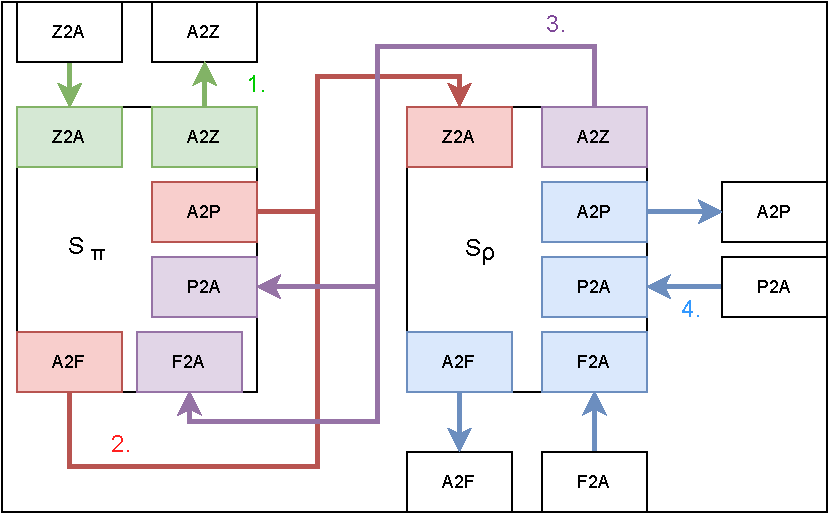
\includegraphics[scale=0.62]{figures/simcomp.pdf}
\caption{The composed simulators for $\F_1 \xrightarrow{\rho \circ \pi} \F_3$. The real world consists of $(\rho \circ \pi, \F_1)$. Inputs from \Z are for $\F_1$ and dummy parties interacting with $\F_1$, which \SIM{\pi} is equipped to handle. Outputs from \SIM{\pi} are for $\F_2$ and dummy parties of $\F_2$ which \SIM{\rho} is equipped to handle. FInally, outputs from \SIM{\rho} are for $\F_3$ and dummy parties of $\F_3$, which is just the ideal world in Theorem~\ref{thm:composition}.}
\label{fig:simcomp}
\end{figure}

%\begin{lstlisting}[basicstyle=\small\BeraMonottFamily, mathescape, frame=single]
%m = recv $\$$p2a ;
%case m (
%  P2A(pid, msg) =>
%   	case msg (
%      Committed =>
%        h = sample r k ;
%        send $\$$z2a P2A2Z(pid, (h)) ;
%      Open(b) =>
%	    x = sample r k ;
%        send $\$$z2a P2A2Z(pid, SMsg(b, x)) ;
%\end{lstlisting}

%When the committer is corrupt, the simulator has to do more work. 
%The key point that makes commitment in the RO model realizable is that \Z acquires commitment to give to the corrupt committer from \Fro through \A. 
%In th ideal world, the simulator recrods all the (key,value) pairs generated by its simulation of \Fro and therefore can always determine the bit \Z is committed to.
%When \Z queries \Sim with \inline{Z2A2F(SHash(b + x))} it stores the value and generates a hash value for it and returns it to \Z. 
%When instructed to give input to the corrupt party the simulator, \Sim gives input \inline{A2P(1, Commit(b))} where $b$ is the bit whos hash was requested.
%
%There is a unique edge case where \Z give some random bit sequence to \S as the commitment which wasn't generated by the random oracle. 
%In this case \S chooses a bit at random annd passes \inline{A2P(1, Commit(b))} to the protocol wrapper where $b$ is randomly selected.
%When prompted to open the commitment, \S does nothing as the real world receiver would fail to confirm whether the commitment corresponds to the bit $b$.




%\subsection{Ideal World}
%We described the functionality \Fcom in detail in Section~\ref{sec:execuc} as well as the functionality wrapper construction around it.
%We now describe how we implement ideal world (dummy) parties.

%We first describe at a high-level, the conversion happening within the functionality wrapper for \Fcom with the \inline{commit} message sent by the sender.
%When the wrapper receives the \inline{commit} message, the functionality wrapper executes the following:
%\begin{lstlisting}[basicstyle=\small\BeraMonottFamily, frame=single, mathescape]
%$\tg{(* l1 : list[pid \textasciicircum sender] *)}$
%case $\$$p2f (
%  yes => 
%    pid = recv $\$$p2f ; msg = recv $\$$p2f ;
%    case msg (
%      Commit(b) => 

%        $\$$ch_ = get_channel_by_pid pid $\$$l1 $\$$l2 ... ;
%        $\$$ch_.commit ;
%        send $\$$ch_ b ;
%        $\$$l2' <- append $\$$ch_ $\$$l2 ;
%\end{lstlisting}
%The wrapper also spawns a process to read from each of \Fcom's outgoing channels, case analyze on their value and send out the corresponding functional message to the protocol wrapper.

%The \msf{execUC} function in Figure~\ref{lst:execuc} accepts some number of type parameter which it spawns the main channels of the protocol with. 
%Most important out of these channels is the types governing communication between \Z and \A and between \Z and the protocol wrapper.
%If the types for these channel in both worlds aren't the same, even the import token expected, then it is trivial for an environment to distinguish the two worlds.
%It suffices to specify the import type parameters (\inline{p2f}, \inline{f2p}, \inline{z2p}, etc.) to \inline{execUC}.
%\paragraph{The Ideal World Execution}
%We summarize the message types in use by describing the type parameters to the ideal world execution.
%For the ideal, \inline{execUC} is invoked as follows (refer to the \inline{execUC} definition in Figure~\ref{lst:execuc} for what each of the parameters refers to):
%\begin{lstlisting}[basicstyle=\small\BeraMonottFamily, frame=single, mathescape]
%$\Type$ z2amsg[a][b] = Z2A2P of pid ^ a 
%                     | Z2A2F of b ;
%$\tg{(* ideal world *)}$
%execUC[K1,K2][comf2p][comp2f][comp2f][comf2p]
%  [comf2p][comp2f][comf2a][coma2f][rof2a][roa2f]
%  [rof2p][rop2f]
%\end{lstlisting}
%%$\tg{(* real world *)}$
%%execUC[K1,K2][comf2p][comp2f][rop2f][rof2p]
%%  [rof2p][rop2f][comf2a][coma2f][rof2a][roa2f]
%%  [rof2p][rop2f]
%Notice that the message types over \inline{p2z} and over \inline{p2f} are the same, because the ideal world parties are dummy parties which simply forward the messages to \Fcom.
%The type parameters for the adversary in the ideal world, though, still take the form of the types of \Fro.
%This is because the inputs \Z gives to both worlds (the dummy adversary in the real world) is intended for \Fro when communicating with the functionality through the adverasary or through corrupt parties 
%
%The party inputs from \inline{a2p} in the ideal world are intended for \Fcom, not \Fro, so they are of the same type \inline{comp2f}.
%Similarly, output from corrupt parties to the adversary in the ideal world is the same as output from \Fcom, and, therefore the message type is the same as \inline{comf2p}.
%The messages type parameters are wrapped in channel-specific types as well.
%For example, the channel \inline{z2a} is typed as follows:
%\begin{lstlisting}[basicstyle=\small\BeraMonottFamily, frame=single, mathescape]
%type z2amsg[a][b] = Z2A2P of pid ^ a
%                      | Z2A2F of b ;
%#z_to_a: comm[z2amsg[a2p][a2f]]
%$\tg{(* a2p=rop2f, a2f=roa2f in execUC above*)}$
%\end{lstlisting}
%
%\paragraph{Ideal Protocol}
%The ideal world protocl is a dummy party which forwards all messages to the functionality. 
%The message content from \inline{z2p} and \inline{p2f} is the same in the ideal world, but it is wrapped in different parameteric typed when it is sent from the \inline{z} or \inline{p}.
%As shown below the messages themselves are the same (\inline{comp2f} but typed differently (\inline{z2pmsg} vs \inline{p2fmsg}):
%\begin{lstlisting}[basicstyle=\small\BeraMonottFamily, frame=single, mathescape]
%$\Type$ z2pmsg[a] = Z2P of pid ^ a ;
%$\Type$ p2fmsg[a] = P2F of pid ^ a ;
%#z_to_p: comm[z2pmsg[comp2f]] ;
%#p_to_f: comm[p2fmsg[comp2f]] ;
%\end{lstlisting}
%The protocol wrapper only needs to forward the message unaltered but using a different type construtor. 

%The ideal functionality \Fcom is the same one introduced in Figure~\ref{fig:fcom} in Section~\ref{sec:nomosuc}. 
%In FIgure~\ref{lst:fcom} we present the Nomos definition of the same functionality and provide the channel types in FIgure~\ref{fig:fcomtypes}.
%We elide some of the clutter of acquiring and releasing shared channels in the form of: \texttt{\$p2f $\leftarrow$ acquire \#p\_to\_f} for clarity. 
%Wherever a linear channel like \texttt{\$p2f} is used it is in fact an acquired shared channel \texttt{\#p\_to\_f}.
%
%The key difference to note between \Fcom and its Nomos version is that the functionality is split up into two processes rather than compressed into one.
%This design decision is required because of how Nomos cycles between processes in a round-robin fashion and the communicator design.
%Therefore, processes must recurse when there is no message to be read and move to the next processes after the first expected message is received--in this case the \msf{P2FCommit(b)} message.
%
%
%\begin{figure}
%\centering
%\msf{type} \msf{Ip2f} = \msf{P2FCommit} of \msf{Bit} | \msf{P2FOpen}
%
%\msf{type} \msf{If2p} = \msf{F2PCommit} | \msf{F2POpen} of \msf{Bit}
%
%\msf{type} \msf{Ip2f} = \msf{SCommit} of Bit | \msf{SOpen}
%
%\msf{type} \msf{If2p} = \msf{RCommit} | \msf{ROpen} of Bit
%
%\msf{type} \msf{Rp2f} = \msf{SHash} of \msf{Int} | \msf{Send} of \msf{pid} \textasciicircum \msf{pid} \textasciicircum \msf{Int}
%
%\msf{type} \msf{Rf2p} = \msf{Pre} of \msf{Int} | \msf{RHash} of \msf{Int} | \msf{MSG} of \msf{pid} \textasciicircum \msf{pid} \textasciicircum \msf{Int}
%
%\caption{Types for the channels in the ideal world for \Fcom. Notice that Ip2f and If2p is the type of the channels \msf{z2p} and \msf{p2z} as they much match for both worlds and the ideal world parties simply forward messages to the functionality. The \msf{p2f} and \msf{f2p} channels are specific to the real and ideal world as the functionalities are not the same. Hence the real-world \msf{p2f} is typed with \msf{Rp2f} for the random oracle and the ideal world \msf{p2f} is typed with \msf{Ip2f} for \Fcom.}
%\label{fig:fcomtypes}
%\end{figure}
%
%\begin{figure*}
%\begin{lstlisting}[basicstyle=\small\BeraMonottFamily]
%proc F_code:
%  (s: sid), (k: Int), (rng: [Bit]), (clist: list[Int]),
%  (#p_to_f: comm[pid ^ Ip2f]{Ip2fn}), (#f_to_p: comm[pid ^ If2p]{If2pn}),
%  (#a_to_f: comm[Ia2f]{Ia2fn}), (#f_to_a: comm[If2a]{If2an})  |- ($ch: FtOE) =
%{
%  case $p2f (
%    yes =>	
%      pid, msg = recv $p2f ;
%      get $pwf {Ip2fn} ;
%      case msg (
%        P2FCommit(b) =>	
%          if pid == 1
%          then
%            send F2PCommit $f2p ;
%            pay {If2pn} $f2p ;
%            $ch <- F_com_open s k rng clist #p_to_f #f_to_p b ;
%          end
%      )
%   | no =>  
%       $ch <- F_code s k rng clist #p_to_f #f_to_p ;
%  )
%}
%
%proc F_code_open:
%{
%  case $p2f (
%    yes =>	
%      pid, msg = recv $p2f ;
%      get $p2f {0} ;
%      case msg (
%        P2FOpen =>	
%          if pid == 1
%          then
%            send F2POpen(b) $f2p ;
%            pay {0} $f2p ;
%            $ch <- 1 ;
%          end
%      )
%   | no =>
%       $ch <- F_code_open s k rng clist #p_to_f #f_to_p b ;
%  )
%}
%\end{lstlisting}
%\end{figure*}
%
%The real world protocol for commitment follows a simple communication patter:
%\begin{enumerate}
%\item On input bit $(\msf{P2FCommit}\ b)$ from the environment, the committer queries the random oracle with the message $(\msf{SHash}\ b | r)$ where $r \xleftarrow{\$} \{0,1\}^k$.
%The returned ``hash value'' is sent to the receiver as the commitment.
%\item On input \msf{P2FOpen} from \Z, the committer sends $(\msf{Send}\ p_L\ b\ r)$ to the receiver.
%\item The receiver checks that the commitment is correct be querying \Fro in the same way and asserting that the has returned $(\msf{RHash}\ h)$ is the same as the one sent by $p_C$.
%\item \todo{the type of Rf2p is kind of wrong so need to correct it}
%\end{enumerate}
%
%We provide only a simulator for the dummy adversary as that guarantees a simulator for all adversaries required our emulation definition.
%The simulator for commitment is relatively simple so we only provide a high-level description here and leave the full simulator code to the appendix.
%The simulator internally simulats the random oracle by maintaining a table of key-value pairs that it can control entirely.
%If the committer is corrupt:
%\begin{enumerate}
%\item The simulator can not determine the bit \Z wants to commit to so selects a random bit when activatd by the environment and gives it as input to the corrupted committer.
%\item When it's asked to open the commitment it simply forwards the request to the corrupt committer and stops.
%\end{enumerate}
%If the receiver is corrupt:
%\begin{enumerate}
%\item When activated by the receiver with (\msf{F2PCommit}), the simulator generates some random string $h$ to represent the commitment, stores it, and sends ($\msf{P2A}\ \msf{MSG}(p_C, p_R, h)$) to \Z.
%\item When it receives ($\msf{F2POpen}\ b$) from the receiver, it returns $(\msf{P2A}\ \msf{MSG}(p_C, p_R, b, r)$ to \Z where $r$ is a randomly generated sequence keeping the pair $(b | r, h)$ as the corresponding entry in the table.
%\item When activated by \Z to check the commitment, \Sim simply returns the commitment hash or creates a new one.
%\end{enumerate}
%
%\paragraph{Simulator Well-Matched}
%It is immediately obvious that the constructed simulator is well-typed if the dummy adversary is well-typed with the given type parameters.
%The simulator receives 1 import token per activation from \Z which suffices to simulated \Fro internally. 
%Subsequently, \Sim keeps all of the import it receives, and, therefore when one of the partiesis corrupt a simple bounding polynomial can be given as:
%\[
%	T_{\Dummysim}(n) = T_{\Fro}(n) + O(1)
%\]
%where $T_{\Fro}$ is a satisfying polynomial for \Fro. The additional constant factor simply accounts for sending messages to the corrupt parties.
%Therefore,
%\begin{gather}
%	\forall \Z, \langle \Z \leftrightarrow \DA \rangle \Rightarrow \langle \Z \leftrightarrow \Dummysim \rangle
%\end{gather}
%
%
%\begin{figure*}
%\begin{lstlisting}[basicstyle=\BeraMonottFamily]
%(* Z2P interface *)
%type Ip2f = P2FCommit of Bit | P2FOpen ;
%type If2p = F2PCommit | F2POpen of Bit ;
%
%(* Ideal World *)
%type Ip2f = SCommit of Bit | SOpen ;
%type If2p = RCommit | ROpen of Bit ;
%
%type Ia2f = 0 ;
%type If2a = 0 ;
%
%type Ia2p = Ip2f ;	(* crupt input is same as z2p *)
%type Ip2a = If2p ;
%
%(* Real World *)
%type Rp2f = SHash of Int | Send of pid ^ pid ^ Int ;
%type Rf2p = Pre of Int | RHash of Int | MSG of pid ^ pid ^ Int ;
%
%type Ra2f = A2Hash of Int ;
%type Rf2a = Hash2A of Int ;
%
%type Ra2p = Rp2f ;
%type Rp2a = Rf2p ;
%
%(* the import here is given as those for the dummy adversary in the real world *)
%p2zn <- 0 ; z2pn <- 1 ;
%a2zn <- 0 ; z2an <- 1 ; 
%
%Rf2pn <- 0 ; Rp2fn <- 1 ;
%Rp2an <- 0 ; Ra2pn <- 1 ;
%Rf2an <- 0 ; Ra2fn <- 1 ;
%
%If2pn <- 0 ; Ip2fn <- 0 ;
%Ip2an <- 0 ; Ia2pn <- 0 ;
%I
%
%(* channels *)
%#z_to_p <- comm[pid ^ Ip2f]
%#p_to_z <- comm[pid ^ If2p]
%#z_to_a <- comm[ z2d[Ra2p][Ra2f] ] ;
%#z_to_z <- comm[ d2z[Rp2a][Rf2a] ] ;
%
%
%(* Real World exec PI *)
%execUC[Ip2f][If2p][Rp2f][Rf2p][Rp2a][Ra2p][Rf2a][Ra2f][a2z][z2a]
%	  {p2zn}{z2pn}{f2pn}{p2fn}{p2an}{a2pn}{f2an}{a2fn}{a2zn}{z2an}
%
%(* Ideal world exec PHI *)
%execUC[If2p][Ip2f][Ip2f][If2p][Ip2a][Ia2p][If2a][Ia2f][a2z][z2a]
%	  {p2zn}{z2pn}
%
%
%
%
%
%
%\end{lstlisting}
%\end{figure*}


The type system in NomosUC helps to identify when the amount of potential that a functionality requires isn't satisfied by the bounding polynomia given.
We illustrate this point using the $\F_{\msf{map}}$. 
The functionality maintains a list that parties can append to the end of or read from.


%\caption{The $\mathcal{F}_{\msf{comm}}$ commitment ideal functionality in Nomos. The types for the sender and receiver channel define what inputs they can give to the functionality and what messsages are sent from the functionality back to the receiver.}
%\label{fig:nomos:commitment}
%\end{figure*}

